\section{Discussion}\label{discussion}

Integrating RL with DBR reduced inventory and shortened throughput
times, thereby increasing production system efficiency by treating the
shipping buffer (SB) as both WIP and FG. From a TOC standpoint, lower
inventory boosts return on investment (ROI) and strengthens cash flow
(Gupta \emph{et al.}, 2002; Machado \emph{et al.}, 2023). It also
mitigates system variability by reducing queues at the resources
(Goldratt, 2006a; Machado \emph{et al.}, 2023). Shorter queues, in turn,
improve lead times, allowing for quicker responses to demand
fluctuations and machine breakdowns (Thürer \emph{et al.}, 2022). By
decomposing the SB into WIP and FG, this approach eliminates the need to
maintain a fixed SB reference value and continuously adjust it,
ultimately streamlining decision-making and enhancing production
efficiency.

The principles of TOC were instrumental in shaping the RL model,
particularly in defining the state and reward function. Since the state
must provide all the information for the agent to make decisions (Sutton
and Barto, 2018), incorporating the SB concept enables the RL agent to
effectively understand the system\textquotesingle s production needs and
meet demand. This approach eliminates the need for comprehensive
monitoring of the production system, such as tracking queued products
(Shiue \emph{et al.}, 2020; Thomas \emph{et al.}, 2018), order
characteristics (Liu \emph{et al.}, 2022; Marchesano \emph{et al.},
2022), or the status and utilization of resources (Liu \emph{et al.},
2022; Sakr \emph{et al.}, 2023). Furthermore, the reward function,
designed based on TOC performance metrics (gain and inventory), has
proven sufficient for training the RL algorithm and has demonstrated its
effectiveness in decision-making.

Typically, RL scheduling methods are limited to scheduling predefined
production orders (Esteso \emph{et al.}, 2023). However, integrating RL
with DBR allows the agent to determine order sizes while scheduling
production based on the volume of finished goods in stock. This approach
adapts RL to a make-to-stock (MTS) environment, contrasting with the
more common focus on make-to-order (MTO) systems (Panzer and Bender,
2022). It also increases the autonomy of the scheduling process,
aligning with the aim of autonomous decision-making in Industry 4.0 (Jan
\emph{et al.}, 2023; Oztemel and Gursev, 2020). Although DBR scheduling
performed effectively in the simulation model, its integration with RL
achieved equivalent productivity while reducing both inventory and
throughput time (\colorbox{yellow!40}{}\hyperref[_Ref187517192]{Table 3}).

Correlation analysis, linear regression, and decision trees were used to
explain the RL agent's decisions, with DBR serving as a baseline for
comparison. These methods confirmed that DBR's behavior aligns with its
underlying model, highlighting how SB levels influence product quantity
decisions (Schragenheim, 2010c). In contrast, the RL agent prioritizes
WIP more than FG when deciding what quantities to produce, showing a
result of RL's capacity to learn the system's dynamics and adapt to
disruptions such as machine breakdowns. This phenomenon is illustrated
in \hyperref[_Ref187517040]{Figure 10}. When resource III experiences a
breakdown (red bar at time T2), parts accumulate in front of the
resource while the market continues to consume the FG. As FG levels
decrease, a new order is released to restore the SB level, leading to an
increase in WIP (time T3). By times T4 and T5, the levels of WIP and FG
return to their initial values due to the protective capacity of the
resources, and product releases continue in accordance with the SB
level.

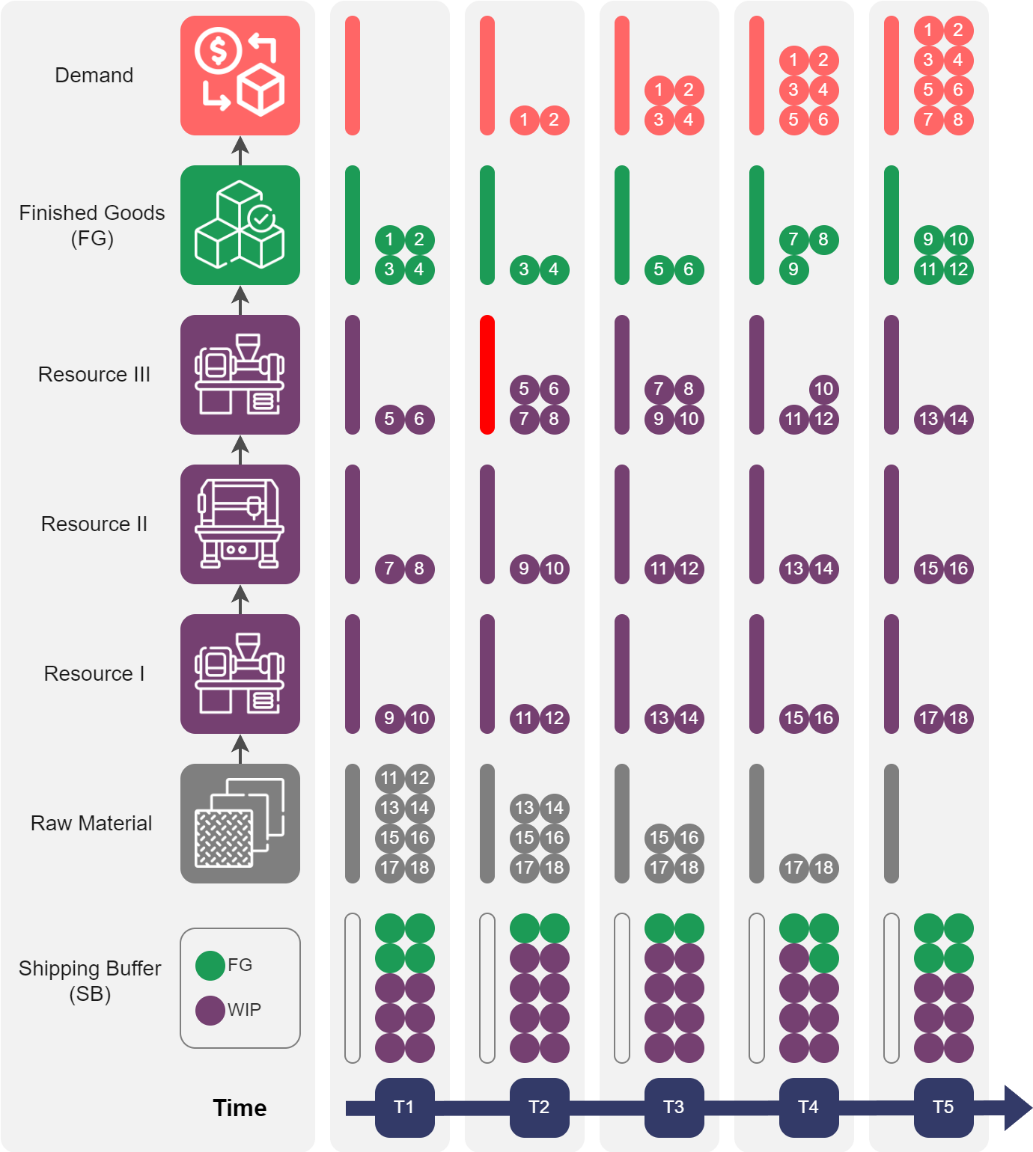
\includegraphics[width=4.68918in,height=5.23285in,alt={Diagrama Descrição gerada automaticamente com confiança baixa}]{figures/fig10.png}

\protect\phantomsection\label{_Ref187517040}{}Figure 10. Machine
breakdown in the DBR.

By highlighting RL\textquotesingle s performance, it becomes evident
that there is potential for improving DBR, particularly by considering
WIP as a standalone decision-making variable rather than treating it
solely as part of the SB. Although no direct relationship between WIP
and the number of products released was identified, the decision tree's
node count reveals a significant difference between the two scheduling
methods. This discrepancy suggests that other variables or combinations
of variables may influence decisions in certain system states. However,
defining these relationships comprehensively can be both labor-intensive
and, in some cases, infeasible (Kuhnle \emph{et al.}, 2022; Rudin
\emph{et al.}, 2022).
